\documentclass[dvipsnames,14pt,t,xelatex]{beamer}
\usepackage{beamerthemeplaincu}
\usepackage{fontenc,xltxtra,xunicode}
\defaultfontfeatures{Mapping=tex-text}
\usepackage[absolute,overlay]{textpos}
\usepackage{graphicx} 
\usepackage[official]{eurosym}
\usepackage[absolute,overlay]{textpos}

%\makeatletter
%\lst@CCPutMacro\lst@ProcessOther {"2D}{\lst@ttfamily{-{}}{-{}}}
%\@empty\z@\@empty
%\makeatother

% beamer stuff 
\renewcommand{\slidecaption}{14.~July 2014}


\begin{document}

%%%%%%%%%%%%%%%%%%%%%%%%%%%%%%%%%%%%%%%%%%%%%%%%%%%%%%%%%%%%%%%%%
\mode<presentation>{
\begin{frame}<1>[t]
\frametitle{%
  \begin{tabular}{@ {}c@ {}}
  \\[4mm]
  \LARGE ITP 2015 will be in Nanjing \\[-2mm] 
  \end{tabular}}

  \begin{center}
  \begin{tabular}{l@{\hspace{2mm}}l}
  organised by & Xingyuan Zhang\\ 
               & Christian Urban
  \end{tabular}
  \end{center}

  \normalsize
  \begin{center}
  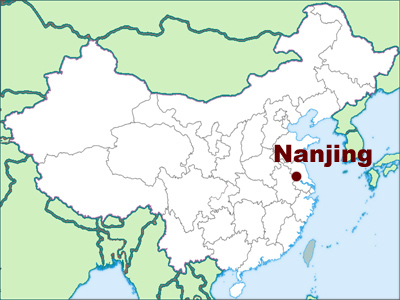
\includegraphics[scale=0.3]{../pics/nanjing-map.jpg}
  \end{center}

\begin{textblock}{7}(12.5,5)
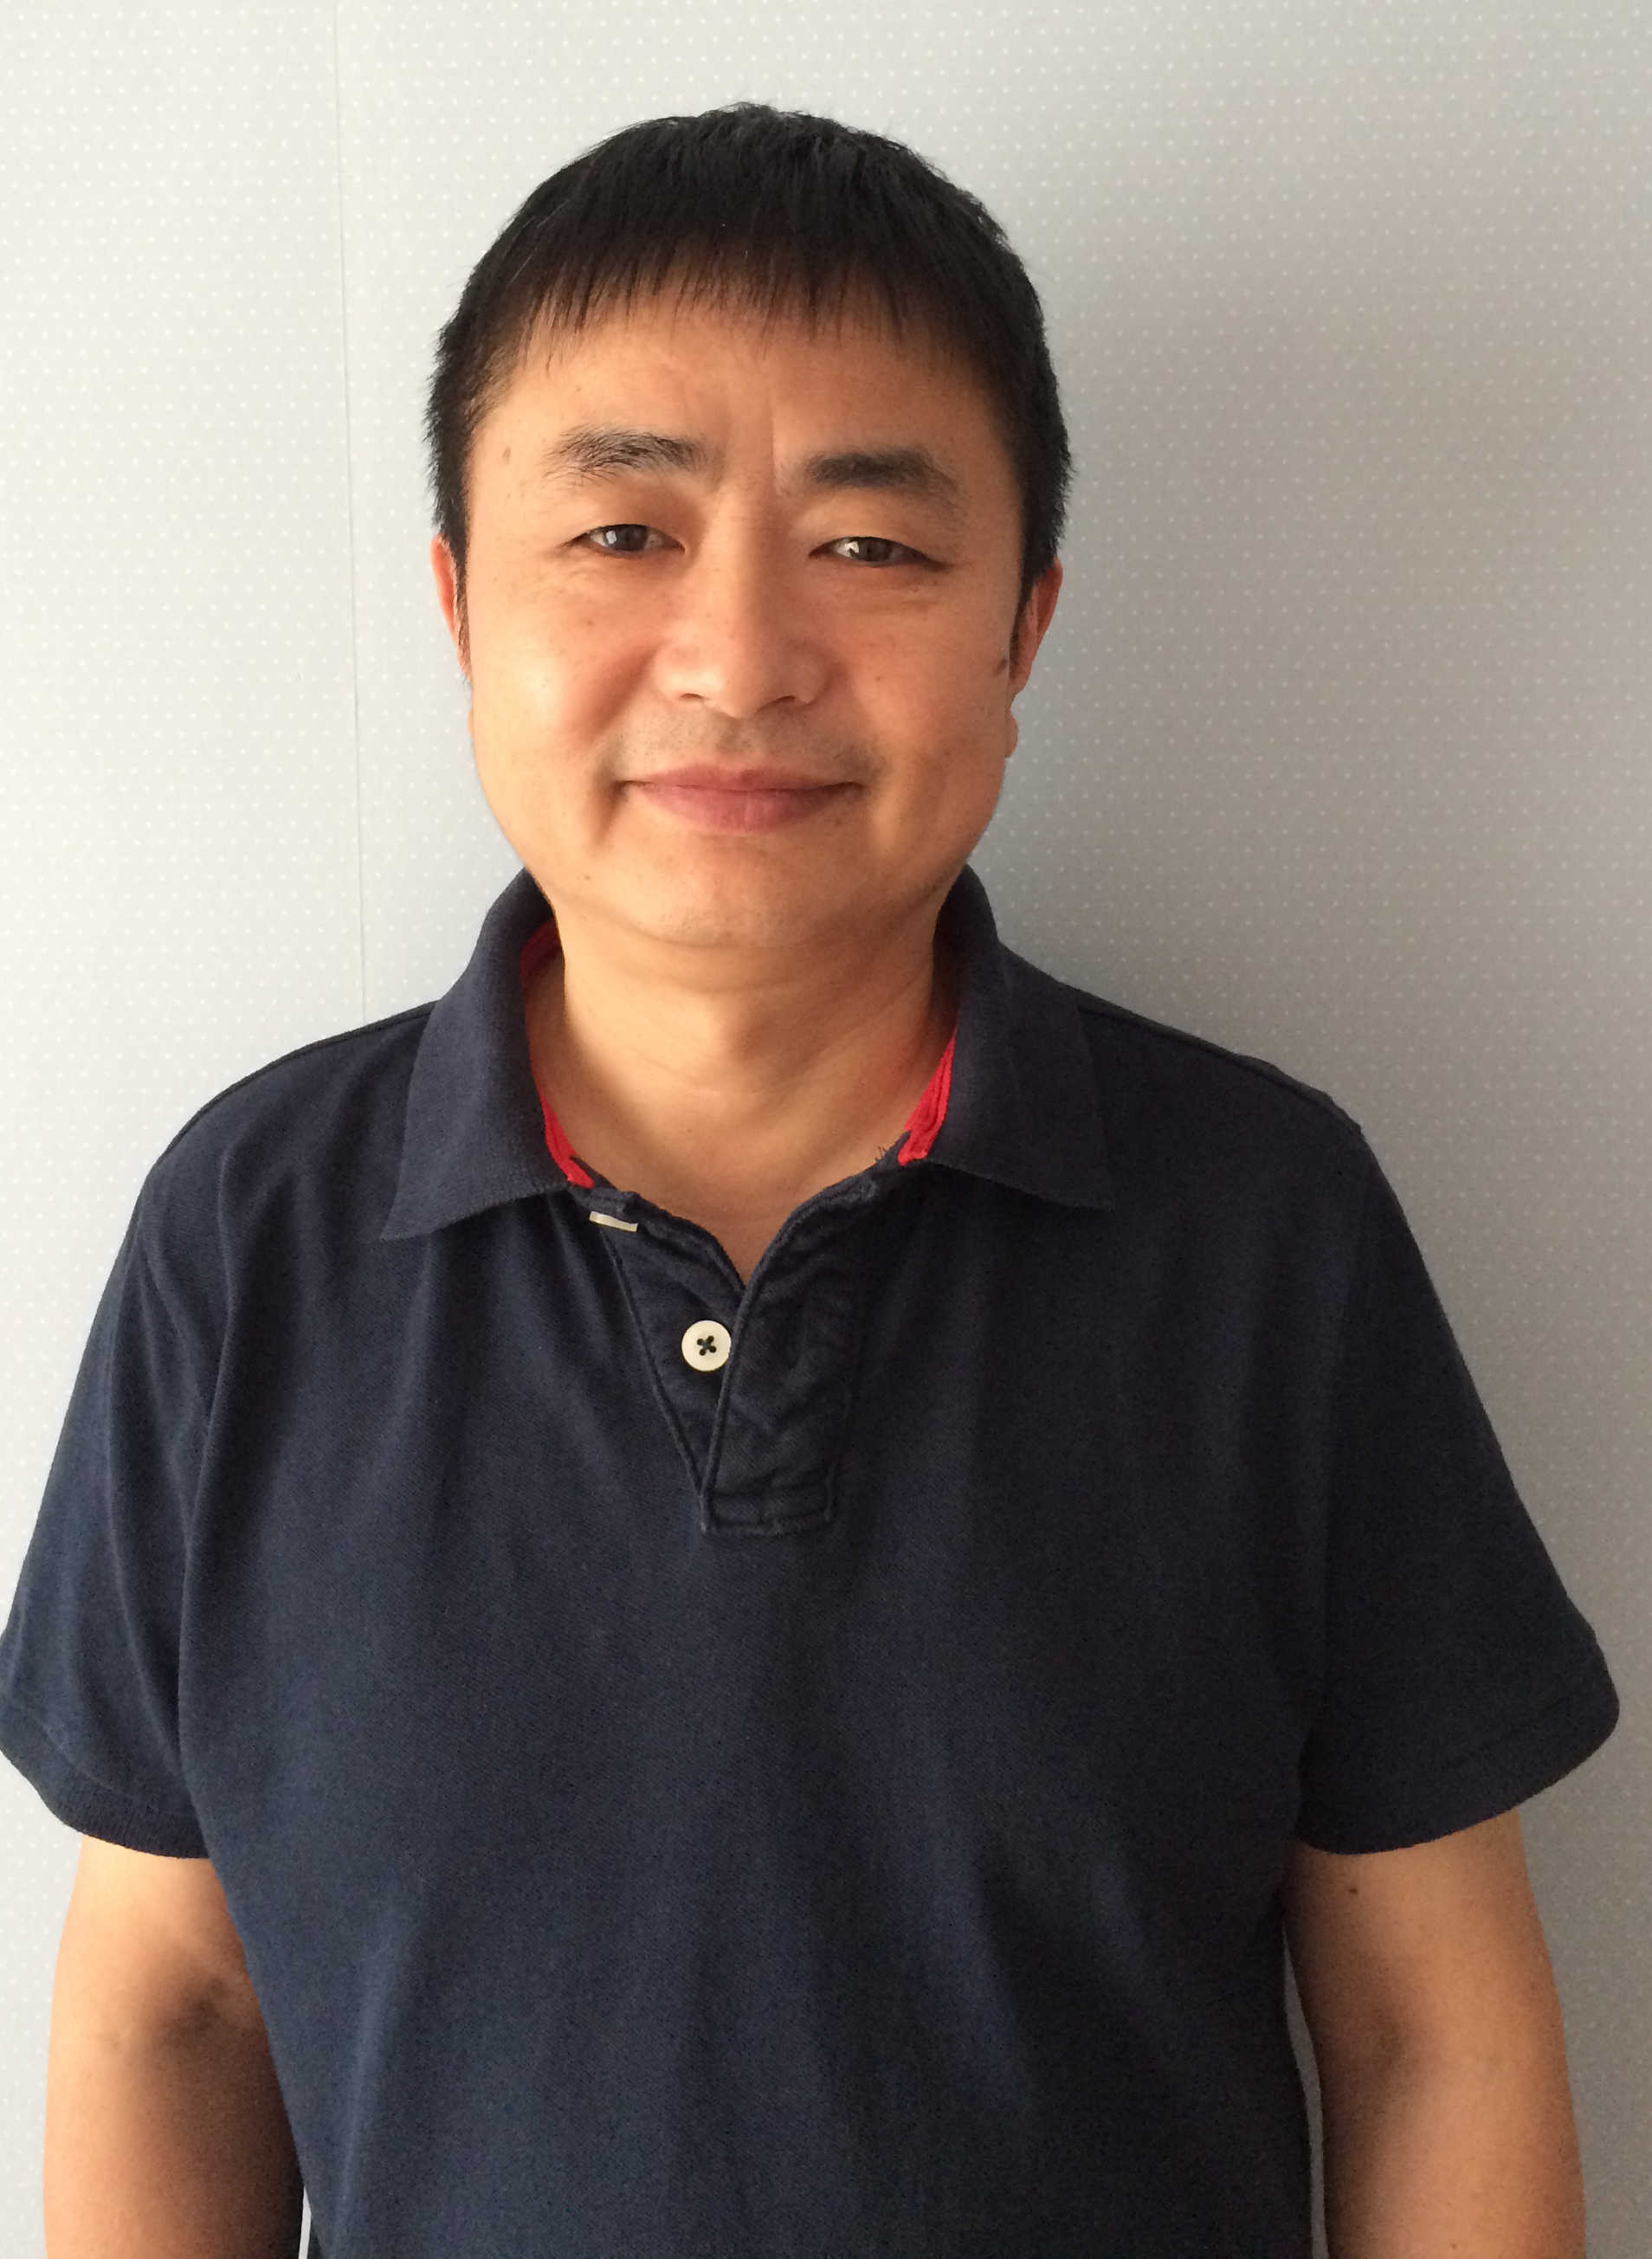
\includegraphics[scale=0.05]{../pics/xingyuan.jpg}
\end{textblock}

\begin{textblock}{7}(10,14.3)
24 - 27 August 2015
\end{textblock}
\end{frame}}
 %%%%%%%%%%%%%%%%%%%%%%%%%%%%%%%%%%%%%%%%%%%%%%%%%%%%%%%%%%%%%%%%%%     


%%%%%%%%%%%%%%%%%%%%%%%%%%%%%%%%%%%%%%%%%%%%%%%%%%%%%%%%%%%%%%%%%%
\mode<presentation>{
\begin{frame}[c]
\frametitle{Travel}


  \begin{center}
  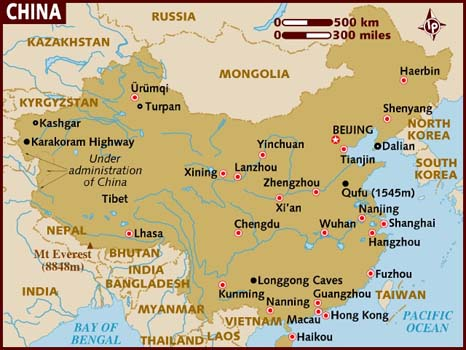
\includegraphics[scale=0.4]{../pics/map_of_china.jpg}
  \end{center}

  direct flights to Nanjing; otherwise stop in 
  Beijing or Hong Kong; or fly to Shanghai and then 
  take the train; take taxis inside Nanjing
\end{frame}}
%%%%%%%%%%%%%%%%%%%%%%%%%%%%%%%%%%%%%%%%%%%%%%%%%%%%%%%%%%%%%%%%%%     

%%%%%%%%%%%%%%%%%%%%%%%%%%%%%%%%%%%%%%%%%%%%%%%%%%%%%%%%%%%%%%%%%%
\mode<presentation>{
\begin{frame}[t]
\frametitle{Hanyuan Hotel}


  \begin{center}
  \begin{tabular}{cc}
  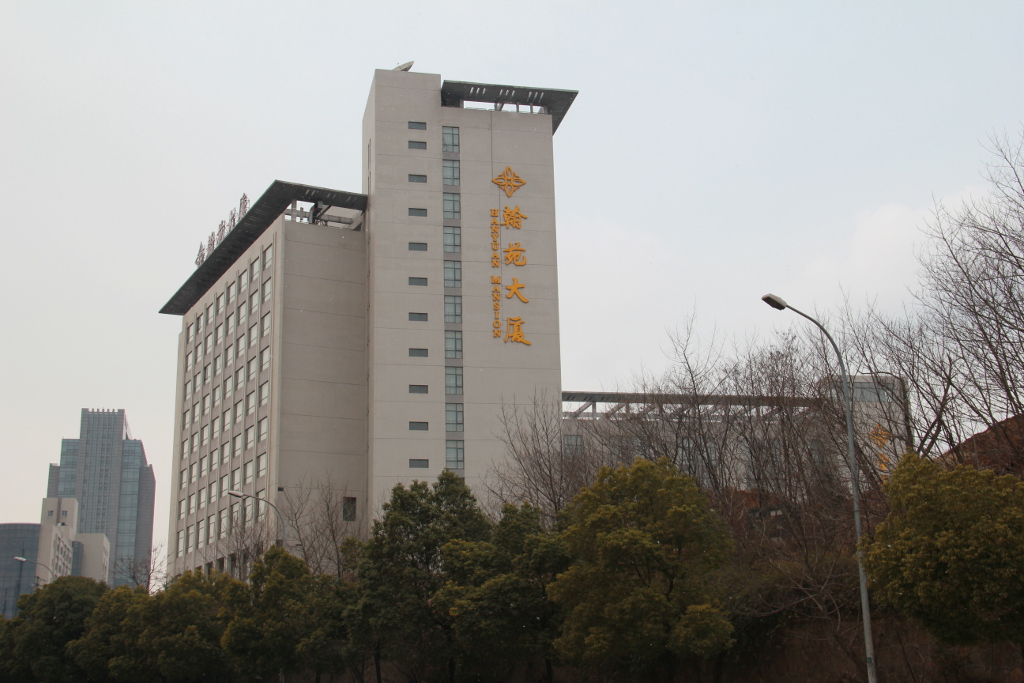
\includegraphics[scale=0.1]{../pics/hotel1.jpg} &
  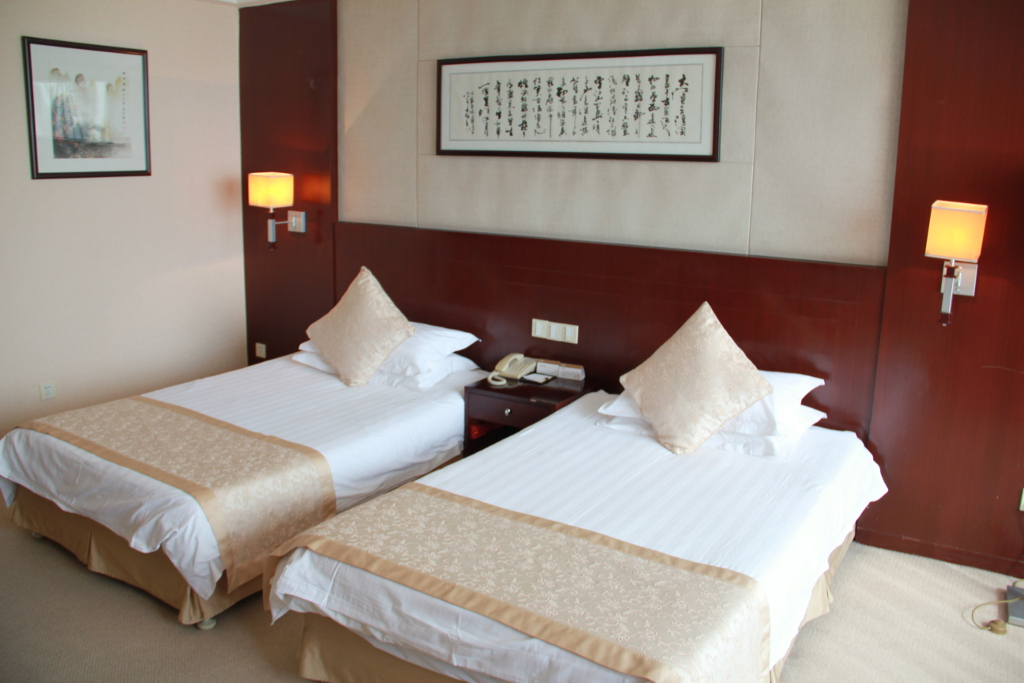
\includegraphics[scale=0.1]{../pics/hotel2.jpg}\\
  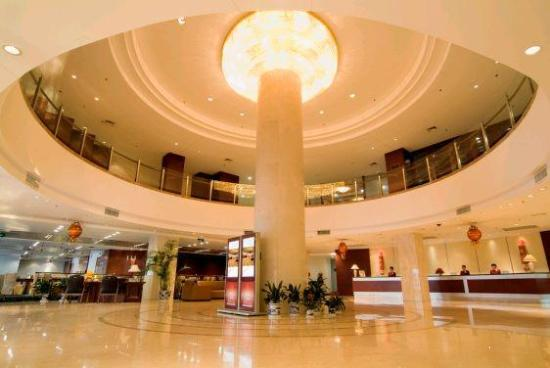
\includegraphics[scale=0.255]{../pics/hotel3.jpg} &
  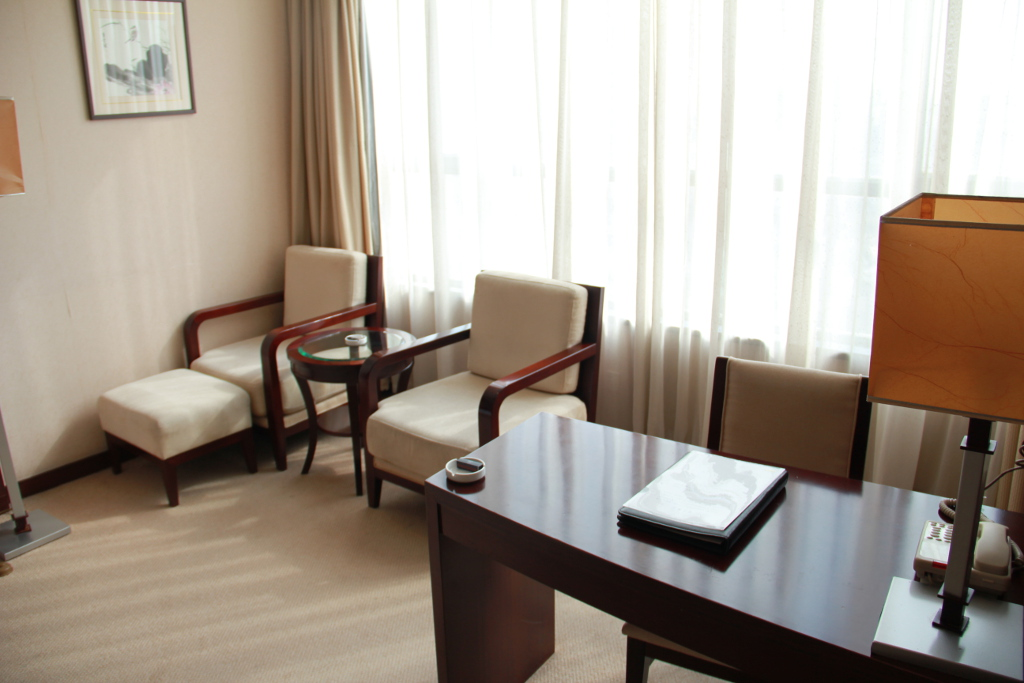
\includegraphics[scale=0.1]{../pics/hotel4.jpg}
  \end{tabular}
   \end{center}

\pounds{35}/\$60/\euro{40} per night, free wifi, includes a 
restaurant, close to universities and downtown  
\end{frame}}
%%%%%%%%%%%%%%%%%%%%%%%%%%%%%%%%%%%%%%%%%%%%%%%%%%%%%%%%%%%%%%%%%%     
%%%%%%%%%%%%%%%%%%%%%%%%%%%%%%%%%%%%%%%%%%%%%%%%%%%%%%%%%%%%%%%%%%
\mode<presentation>{
\begin{frame}[t]
\frametitle{Excursion}

\begin{itemize}
\item either to the Slender Westlake in Yangzhou 
\item or the Purple Mountains in Nanjing
\end{itemize}

\begin{center}
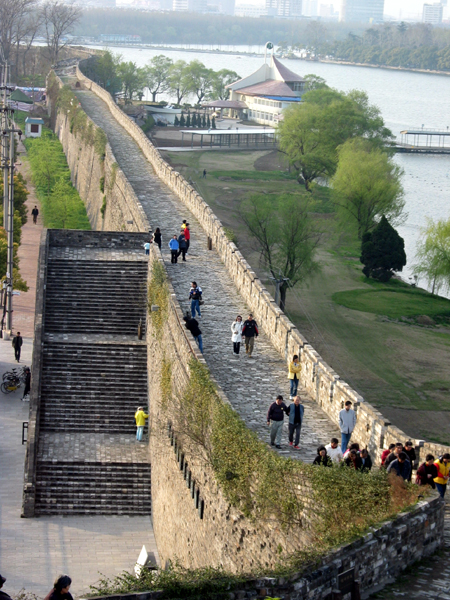
\includegraphics[scale=0.25]{../pics/ITP-najing-cit-walk.jpg}
\hspace{3mm}
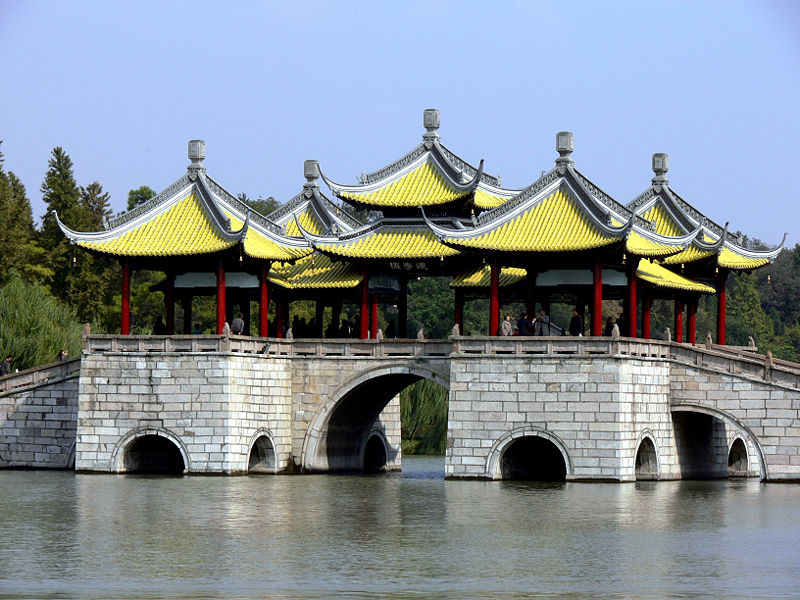
\includegraphics[scale=0.1]{../pics/Yangzhou2.jpg}
\hspace{3mm}
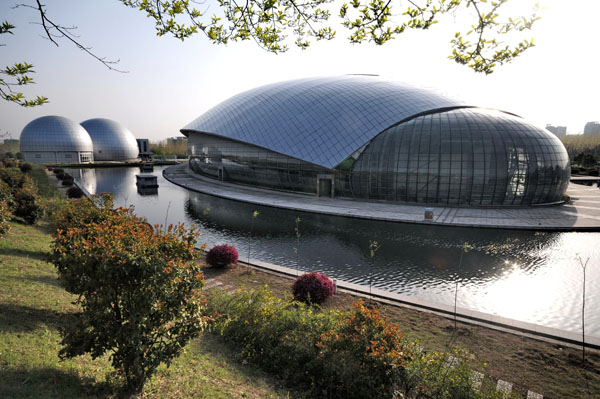
\includegraphics[scale=0.6]{../pics/Nanjing4.jpg}
\end{center}

\end{frame}}
%%%%%%%%%%%%%%%%%%%%%%%%%%%%%%%%%%%%%%%%%%%%%%%%%%%%%%%%%%%%%%%%%%     


%%%%%%%%%%%%%%%%%%%%%%%%%%%%%%%%%%%%%%%%%%%%%%%%%%%%%%%%%%%%%%%%%%
\mode<presentation>{
\begin{frame}[c]
\frametitle{First ITP in China/Asia}

\begin{itemize}
\item you will need a visa!
\item watch the webpage for travel guidance\medskip\pause
\item any question you already have?\bigskip
\end{itemize}\pause

\begin{center}
\Large\fontspec{Hoefler Text Black}
\textcolor{ProcessBlue}{Welcome to Nanjing next year\\
\large 24 - 27 August 2015
}
\end{center}
\end{frame}}
%%%%%%%%%%%%%%%%%%%%%%%%%%%%%%%%%%%%%%%%%%%%%%%%%%%%%%%%%%%%%%%%%%     



\end{document}

%%% Local Variables:  
%%% mode: latex
%%% TeX-master: t
%%% End: 

